
% This LaTeX was auto-generated from an M-file by MATLAB.
% To make changes, update the M-file and republish this document.

\documentclass{article}
\usepackage{graphicx}
\usepackage{color}
\usepackage{listings}
\usepackage[framed]{mcode}
\usepackage{fullpage}
\usepackage{hyperref}
\usepackage{amsmath}

\definecolor{lightgray}{gray}{0.5}
\setlength{\parindent}{0pt}

\begin{document}

    
    
%\section*{}

\begin{par}

\title{BE 521 - Homework 8\\{\normalsize Spring 2015}}
\author{Mike Lautman}
\date{\today}
\maketitle
\textbf{Objective:} Spell letters using neurosignals

\end{par}
\begin{par}

\section*{0 Setup}

\end{par}
\begin{lstlisting}
clf; close all; clear; clc;
\end{lstlisting}


\subsection*{Setup the SVM package}

\begin{lstlisting}
addpath(genpath('./libsvm-3.20/matlab/')); addpath(genpath('./I521_A0008_D001_Annotations/')); 
cd libsvm-3.20/matlab/ 
make cd ../..
\end{lstlisting}


\subsection*{LOAD EEG data from server}

\begin{lstlisting}
me = 'mlautman'; 
pass_file = 'mla_ieeglogin.bin'; 
dataset1 = 'I521_A0008_D001'; 
[T, session1] = evalc('IEEGSession(dataset1, me, pass_file)'); 
data1 = session1.data; 
sr1 = data1.channels(1).sampleRate; 
nr_samples = 3672000;\%data1.channels(1).getNrSamples; 
n_chan = 64;
\end{lstlisting}
\begin{lstlisting}
neurons = zeros(nr\_samples,n\_chan); for i = 1:n\_chan     neurons(1:nr\_samples, i) = data1.getvalues(1:nr\_samples, i); end
\end{lstlisting}


\subsection*{Load target data}

\begin{lstlisting}
addpath(genpath('./data/'));
addpath(genpath('./I521_A0008_D001_Annotations//'));
load('./I521_A0008_D001_Annotations/TargetLetterAnnots.mat');
load('./I521_A0008_D001_Annotations/StimAnnots.mat');
load('./data/neurons.mat');
\end{lstlisting}
\color{black}


\subsection*{Put mat data into usable form}

\begin{lstlisting}
% grab all data into cell form
T_c = {TargetLetter.description};
S_d_c = {Stim.description};
S_t_c = {Stim.type};
start = cell2mat({Stim.start});
stop = cell2mat({Stim.stop});

%preallocate
N_stim = length(S_d_c);
S_d = zeros(1, N_stim);
S_t = zeros(1, N_stim);
T = zeros(1, 85);

for i=1:N_stim
    S_d(i) = str2num(S_d_c{i});
    S_t(i) = str2num(S_t_c{i});
end

for i=1:85
    T(i) = int64(T_c{i});
end
\end{lstlisting}
\begin{par}

\section*{1 Exploring the Data}

\end{par}
\begin{par}

\subsection*{1.1 Channel 11 mean EEG}

\end{par}
\begin{lstlisting}
channel = 11;
start_hit_i = floor(start(find(S_t)) / 1e6 * 240);
stop_hit_i = floor(stop(find(S_t)) / 1e6 * 240);

start_miss_i = floor(start(find(~S_t)) / 1e6 * 240);
stop_miss_i = floor(stop(find(~S_t)) / 1e6 * 240);

ave_hit = zeros( floor(stop_hit_i(1) - start_hit_i(1)), 1);
ave_miss = zeros( floor(stop_miss_i(1) - start_miss_i(1)), 1);

for i=1:length(start_hit_i)
    ave_hit = ave_hit + neurons(1+start_hit_i(i):stop_hit_i(i), channel);
end
ave_hit = ave_hit / (length(start_hit_i));

for i=1:length(start_miss_i)
    ave_miss = ave_miss + neurons(1+start_miss_i(i):stop_miss_i(i), channel);
end
ave_miss = ave_miss / (length(start_miss_i));
\end{lstlisting}


\subsection*{plot results}

\begin{lstlisting}
time_ms = (1:length(ave_hit))/length(ave_hit) * 1000;
figure(1)
title('Channel 11 Target vs Non-Target Average Response Waveform');
subplot(2,1,1)
plot(time_ms, ave_hit)
title('Target average response')
xlabel('Time (ms)')
ylabel('EEG')
ylim([-10 10])
subplot(2,1,2)
plot(time_ms,ave_miss)
title('Target average response')
xlabel('Time (ms)')
ylabel('EEG')
ylim([-10 10])
\end{lstlisting}


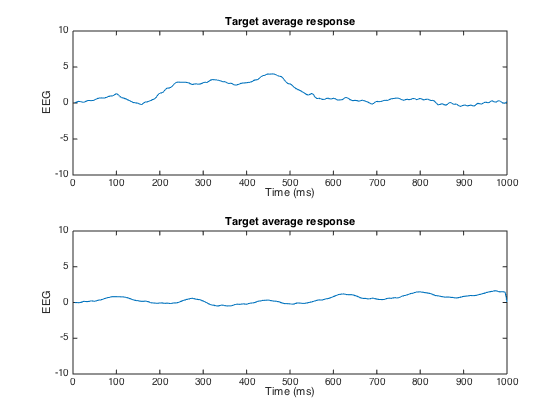
\includegraphics [width=4in]{mlautman_hw8_01.png}
\begin{par}

\subsection*{1.2 Channel 23 mean EEG}

\end{par}
\begin{lstlisting}
channel = 23;
for i=1:length(start_hit_i)
    ave_hit = ave_hit + neurons(1+start_hit_i(i):stop_hit_i(i), channel);
end
ave_hit = ave_hit / (length(start_hit_i));

for i=1:length(start_miss_i)
    ave_miss = ave_miss + neurons(1+start_miss_i(i):stop_miss_i(i), channel);
end
ave_miss = ave_miss / (length(start_miss_i));
\end{lstlisting}


\subsection*{plot results}

\begin{lstlisting}
time_ms = (1:length(ave_hit))/length(ave_hit) * 1000;
figure(2)
title('Channel 23 Target vs Non-Target Average Response Waveform');
subplot(2,1,1)
plot(time_ms, ave_hit)
title('Target average response')
xlabel('Time (ms)')
ylabel('EEG')
ylim([-10 10])
subplot(2,1,2)
plot(time_ms,ave_miss)
title('Target average response')
xlabel('Time (ms)')
ylabel('EEG')
ylim([-10 10])
\end{lstlisting}


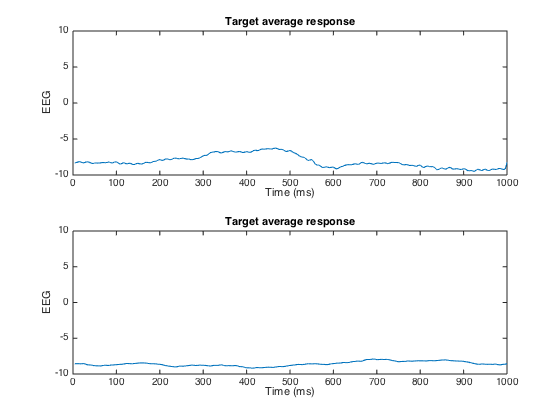
\includegraphics [width=4in]{mlautman_hw8_02.png}
\begin{par}

\subsection*{1.3}
Between the two, It would be significantly easier to use channel 11 than
channel 23. Looking at the differences in amplitude between the average
hit signal and average miss signal, it is clear that channel 11 is far
superior for distinguishing between hits and misses. The largest
difference between hits and misses on channel 11 occurs between 300 and
500 ms after the stimulus.

\end{par}
\begin{par}

\subsection*{1.4 TopoplotEEG}

\end{par}
\begin{lstlisting}
hit = zeros(240, 64);
miss = zeros(240, 64);

for channel = 1:64;
   for i = 1:length(start_hit_i)
       s = 1 + start_hit_i(i);
       e = s + 240 - 1; %stop_hit_i(i);
       hit(:, channel) = hit(:, channel) + neurons(s:e,channel);
   end
   hit(:,channel) = hit(:,channel) / (length(start_hit_i));
   for i = 1:length(start_miss_i)
       s = 1 + start_miss_i(i);
       e = s + 240 - 1; %stop_miss_i(i);
       miss(:, channel) = miss(:, channel) + neurons(s:e,channel);
   end
   miss(:,channel) = miss(:,channel) / (length(start_miss_i));
end
\end{lstlisting}


\subsection*{plot}

\begin{lstlisting}
figure(3)
i = 72;
% for i = 1:240
mean_diff = hit(i, :) - miss(i, :);
topoplotEEG(mean_diff,'eloc64.txt','gridscale',150);
title('TopoPlotEEG of P300 Signal at 300ms after Stimulation');
colorbar;
% pause(1/240)
% end
\end{lstlisting}


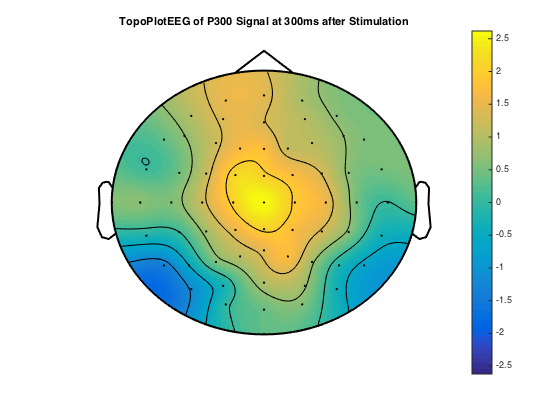
\includegraphics [width=4in]{mlautman_hw8_03.png}
\begin{par}

\subsection*{1.5 TopoplotEEG Analysis}
The topoplotEEG shows that the region corresponding with channel 11 (in
the middle of the head) has the highest delta wheras the areas towards
the front, back, left and right of the head have significantly lower
deltas. Since channel 23 corresponds to a node at the front of the head,
it makes sense that it would be a less accurate predictor.

\end{par}
\begin{par}

\section*{2 Using Individual P300s in Prediction}

\end{par}
\begin{par}

\subsection*{2.1 Advantages and Disadvantages of only using one channel}
Other than the obvious computational speed advandage of using just one
channel, another advantage is transparency of learning algorithm results.
With 64 channels, it is significantly harder to design a learning
algorithm where the learned parameters are easy to visualize. By limiting
the learning algorithm to a single channel, it is significantly easier
interpret the decision surface learned through training. An obvious
disadvantage of using just one channel is by throwing out information, we
limit the complexity of the decision surface learnable by our learning
algorithm. Ultimately, we sacrifice accuracy for easily interpretable
results.

\end{par}
\begin{par}

\section*{2.2 }

\end{par}
\begin{lstlisting}
channel = 11;
epoch = 10;
iteration = 11;

s = ((epoch - 1) * 180 + (iteration - 1)) * 240  + 1;
e = s + 240 - 1;
sample = neurons(s:e, channel);
score_1 = 240 * 0.25;
score_2 = 240 * 0.45;
score_3 = 240 * 0.60;
score_4 = 240 * 0.70;
p300_score = mean(sample(score_1:score_2)) - mean(sample(score_3:score_4))
\end{lstlisting}

\color{lightgray} \begin{lstlisting}
p300_score =

    1.4996

\end{lstlisting} \color{black}
\begin{par}

\section*{2.3 P300 score for each iteration in epoch 20}

\end{par}
\begin{lstlisting}
channel = 11;
epoch = 20;

p300_score = zeros(180,1);
column = zeros(180,1);

for iteration = 1:180
    s = ((epoch - 1) * 180 + (iteration - 1)) * 240  + 1;
    e = s + 240 - 1;
    sample = neurons(s:e, channel);
    p300_score(iteration) = ...
        mean(sample(score_1:score_2)) - mean(sample(score_3:score_4));
    column(iteration) = S_d(iteration + 180 * (epoch - 1));
end

sorted_scores = zeros(15,12);
for i=1:12
    sorted_scores(:,i) = p300_score(column==i);
end

figure(4)
boxplot(sorted_scores)
\end{lstlisting}


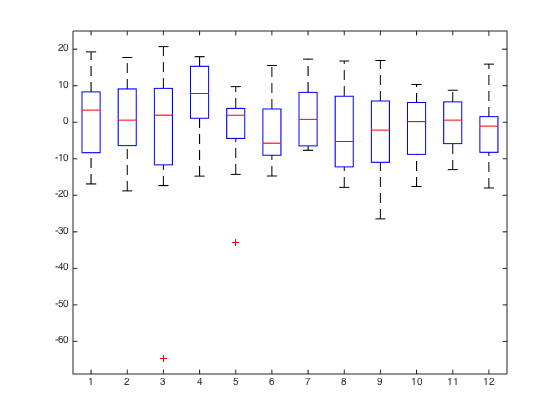
\includegraphics [width=4in]{mlautman_hw8_04.png}
\begin{par}

\section*{2.4  P300 score for each iteration in epoch 20}
Based on the results from 2.3 I would predict column 4 and row 7. Column
4 is the clear winner for columns since it has the highest mean of the
columns 1-6. Row 7 is less obvious however, it does have the highest mean
p300 score.

\end{par}
\begin{par}

\section*{2.5 }
Based on the results from 2.3 I would predict column 4 and row 7. Column
4 is the clear winner for columns since it has the highest mean of the
columns 1-6. Row 7 is less obvious however, it does have the highest mean
p300 score. This gives us the letter D.

\end{par}
\begin{lstlisting}
channel = 11;

ref = [...
    'A' 'B' 'C' 'D' 'E' 'F';
    'G' 'H' 'I' 'J' 'K' 'L';
    'M' 'N' 'O' 'P' 'Q' 'R';
    'S' 'T' 'U' 'V' 'W' 'X';
    'Y' 'Z' '1' '2' '3' '4';
    '5' '6' '7' '8' '9' '_'
];

letters = cell(1, 85);
for epoch = 1:85
    p300_score = zeros(180,1);
    column = zeros(180,1);

    for iteration = 1:180
        s = ((epoch - 1) * 180 + (iteration - 1)) * 240  + 1;
        e = s + 240 - 1;
        sample = neurons(s:e, channel);
        p300_score(iteration) = ...
            mean(sample(score_1:score_2)) - mean(sample(score_3:score_4));
        column(iteration) = S_d(iteration + 180 * (epoch - 1));
    end

    sorted_scores = zeros(15,12);
    for i=1:12
        sorted_scores(:,i) = p300_score(column==i);
    end

    mean_ss = mean(sorted_scores,1);
    [m, col] = max(mean_ss(1:6));
    [m, row] = max(mean_ss(7:12));
    letters{epoch} = ref(row, col);
end

letters
\end{lstlisting}

\color{lightgray} \begin{lstlisting}
letters = 

  Columns 1 through 11

    '4'    'A'    'P'    'V'    '5'    'U'    'F'    'O'    'H'    'I'    'O'

  Columns 12 through 22

    'Q'    'B'    'R'    'J'    'M'    'F'    'C'    'E'    'D'    '_'    'C'

  Columns 23 through 33

    'T'    'W'    'I'    'D'    'B'    'P'    'C'    'O'    'A'    'W'    'R'

  Columns 34 through 44

    '5'    'I'    'U'    'K'    'O'    'L'    '3'    'O'    'O'    'E'    'W'

  Columns 45 through 55

    'E'    '6'    'T'    'G'    'K'    '4'    'R'    'Z'    '3'    'O'    'L'

  Columns 56 through 66

    'H'    'Y'    '6'    'O'    '_'    'E'    'X'    'E'    'K'    'V'    'L'

  Columns 67 through 77

    'N'    'X'    'T'    'K'    'K'    'P'    'I'    'H'    'N'    'T'    'F'

  Columns 78 through 85

    'X'    'X'    'L'    'O'    'T'    'B'    'Q'    'R'

\end{lstlisting} \color{black}


\subsection*{score}

\begin{lstlisting}
pred = zeros(1,85);
for i=1:85
    pred(i) = int64(letters{i});
end
accuracy_2 = sum(pred == T)/length(T);
\end{lstlisting}
\begin{par}

\section*{3. Automating the Learning}

\end{par}
\begin{par}

\subsection*{3.1 play}
After working with the data for sometime, the best accuracy achieved was
in the 50\% range. With more time, I am sure that I would be able to get
that number into the 90\% range.

\end{par}


\subsection*{Convolve with gaussian and Subsample the data}

\begin{lstlisting}
subsample = 1; 
coeff = ones(1,10)/10; 
ss_mask = 1:subsample:size(neurons,1); 
electrode_mask = [3,4,5,10,11,12,17,18,19]; 
neuronMASS = zeros(length(ss_mask), length(electrode_mask));
\end{lstlisting}
\begin{lstlisting}
for i = 1:length(electrode_mask)     
	ch = electrode_mask(i);     
	MA = filter(coeff, 1, neurons(:,ch));     
	neuronMASS(:,i) = MA(ss_mask); 
end
\end{lstlisting}


\subsection*{generate lpf filter}

\begin{lstlisting}
order = 10; 
% Pass band Ripple in dB 
Rp = .01; 
% Stop band Ripple in dB 
Rs = 10; 
% Edge frequency in Hz 
e_f = 3; 
% Normalized Edge frequency in pi * rad/sample 
Wp = e_f / 240 * 2*pi; 
% Design low pass filter 
[b,a] = ellip(order, Rp, Rs, Wp, 'low');
\end{lstlisting}
\begin{lstlisting}
subsample = 1; 
ss_mask = 1:subsample:size(neurons,1); 
electrode_mask = 1:64; 
neuronMASS = zeros(length(ss_mask), length(electrode_mask));
\end{lstlisting}
\begin{lstlisting}
for i = 1:length(electrode_mask)     
	ch = electrode_mask(i);     
	MA = filter(b,a, neurons(:,ch));     
	neuronMASS(:,i) = MA(ss_mask); 
end
\end{lstlisting}


\subsection*{vectorize the testing and training sets}

\begin{lstlisting}
n_vec = reshape(neuron', [240/subsample * length(electrode_mask), 85 * 180])';
\end{lstlisting}
\begin{lstlisting}
% %% separate test and training sets
% s_train = 1;
% e_train = 180*50;
% s_test = e_train + 1;
% e_test = size(n_vec, 1);
%
% neurons_train = n_vec(s_train:e_train, :);
% label_train = S_t(s_train:e_train)';
% neurons_test = n_vec(s_test:e_test, :);
% label_test = S_t(s_test:e_test)';
%
\end{lstlisting}


\subsection*{train a SVM on the p300 scores}

\begin{lstlisting}
model = svmtrain(neurons_train, label_train, 'kernel_function', 'rbf', 'rbf_sigma', 1); 
pred = svmclassify(model, neurons_test); 
svm_model = svmtrain(label_train, neurons_train, '-s 0 -t 2 -b 1');
[predicted_label, accuracy, pred_prob] = svmpredict(label_test, neurons_test, svm_model);
\end{lstlisting}

\begin{lstlisting}
% p300_score = zeros(length(S_t),64);
% column = zeros(length(S_t),1);
% cnt = 0;
%
% for epoch = 1:85
%     for iteration = 1:180
%         cnt = cnt + 1;
%         s = ((epoch - 1) * 180 + (iteration - 1)) * 240  + 1;
%         e = s + 240 - 1;
%         column(cnt) = S_d(iteration + 180 * (epoch - 1));
%         for channel  = 1:64
%             sample = neurons(s:e, channel);
%             p300_score(cnt, channel) = ...
%                 mean(sample(score_1:score_2)) - mean(sample(score_3:score_4));
%         end
%     end
%
%     sorted_scores = zeros(15,12);
%     for i=1:12
%         sorted_scores(:,i) = p300_score(column==i);
%     end
% end
\end{lstlisting}


\subsection*{train a SVM}

\begin{lstlisting}
model = svmtrain(p300_score(1:(50*180),:), S_t(1:(50*180)), 'kernel_function', 'rbf', 'rbf_sigma', 1); 
pred = svmclassify(model, p300_score((50*180+1):(85*180),:));
\end{lstlisting}


\subsection*{AdaBoost with decision Trees}

\begin{lstlisting}
ens=fitensemble(neurons_train, label_train, 'AdaBoostM1',100,'Tree'); 
pred = predict(ens, neurons_test);
\end{lstlisting}
\begin{par}

\subsection*{3.2 method}
For this section I used a SVM with a RBF kernel. For computational ease, I tried two methods to reduce the dimensionality of the feature vector. First I smoothed out the EEG responses using a low pass filter, and then subsampled the smooth signals. Using this method, I was able to preserve the low frequency characteristics of the wave with as few as 24 points per signal. Knowing that some electrodes are more useful than others, I also experimented with different combinations of electrodes. By limiting our scope to the 9 most influential electrodes, we were able to get the feature vector down to a length of 216. A very computationally feasible length. Unfortunately, the svm's had a lot of trouble converging with 9000 training samples. This is most likely due to issues in matlab's implementation of SVMs since similar tests in python converged without issue. In the hopes of getting useful results in matlab, we also applied SVMs to the p300 scores to see if that helped our accuracy over the max mean method. This resulted in an accuracy score in the mid 40\%'s. The third algorithm we tried was AdaBoost with decisiion trees as the base classifier. This method had the higest accuracy yeilding the highest accuracy scores in the low 50\%s.

\end{par}


\subsection*{Clean up}

\begin{lstlisting}
clf; clear all; close all;
\end{lstlisting}



\end{document}
    
